\documentclass{standalone}
\usepackage{tikz}
\usetikzlibrary{patterns, positioning}
\usepackage[sfdefault]{ClearSans} %% option 'sfdefault' activates Clear Sans as the default text font
\usepackage[T1]{fontenc}

\begin{document}
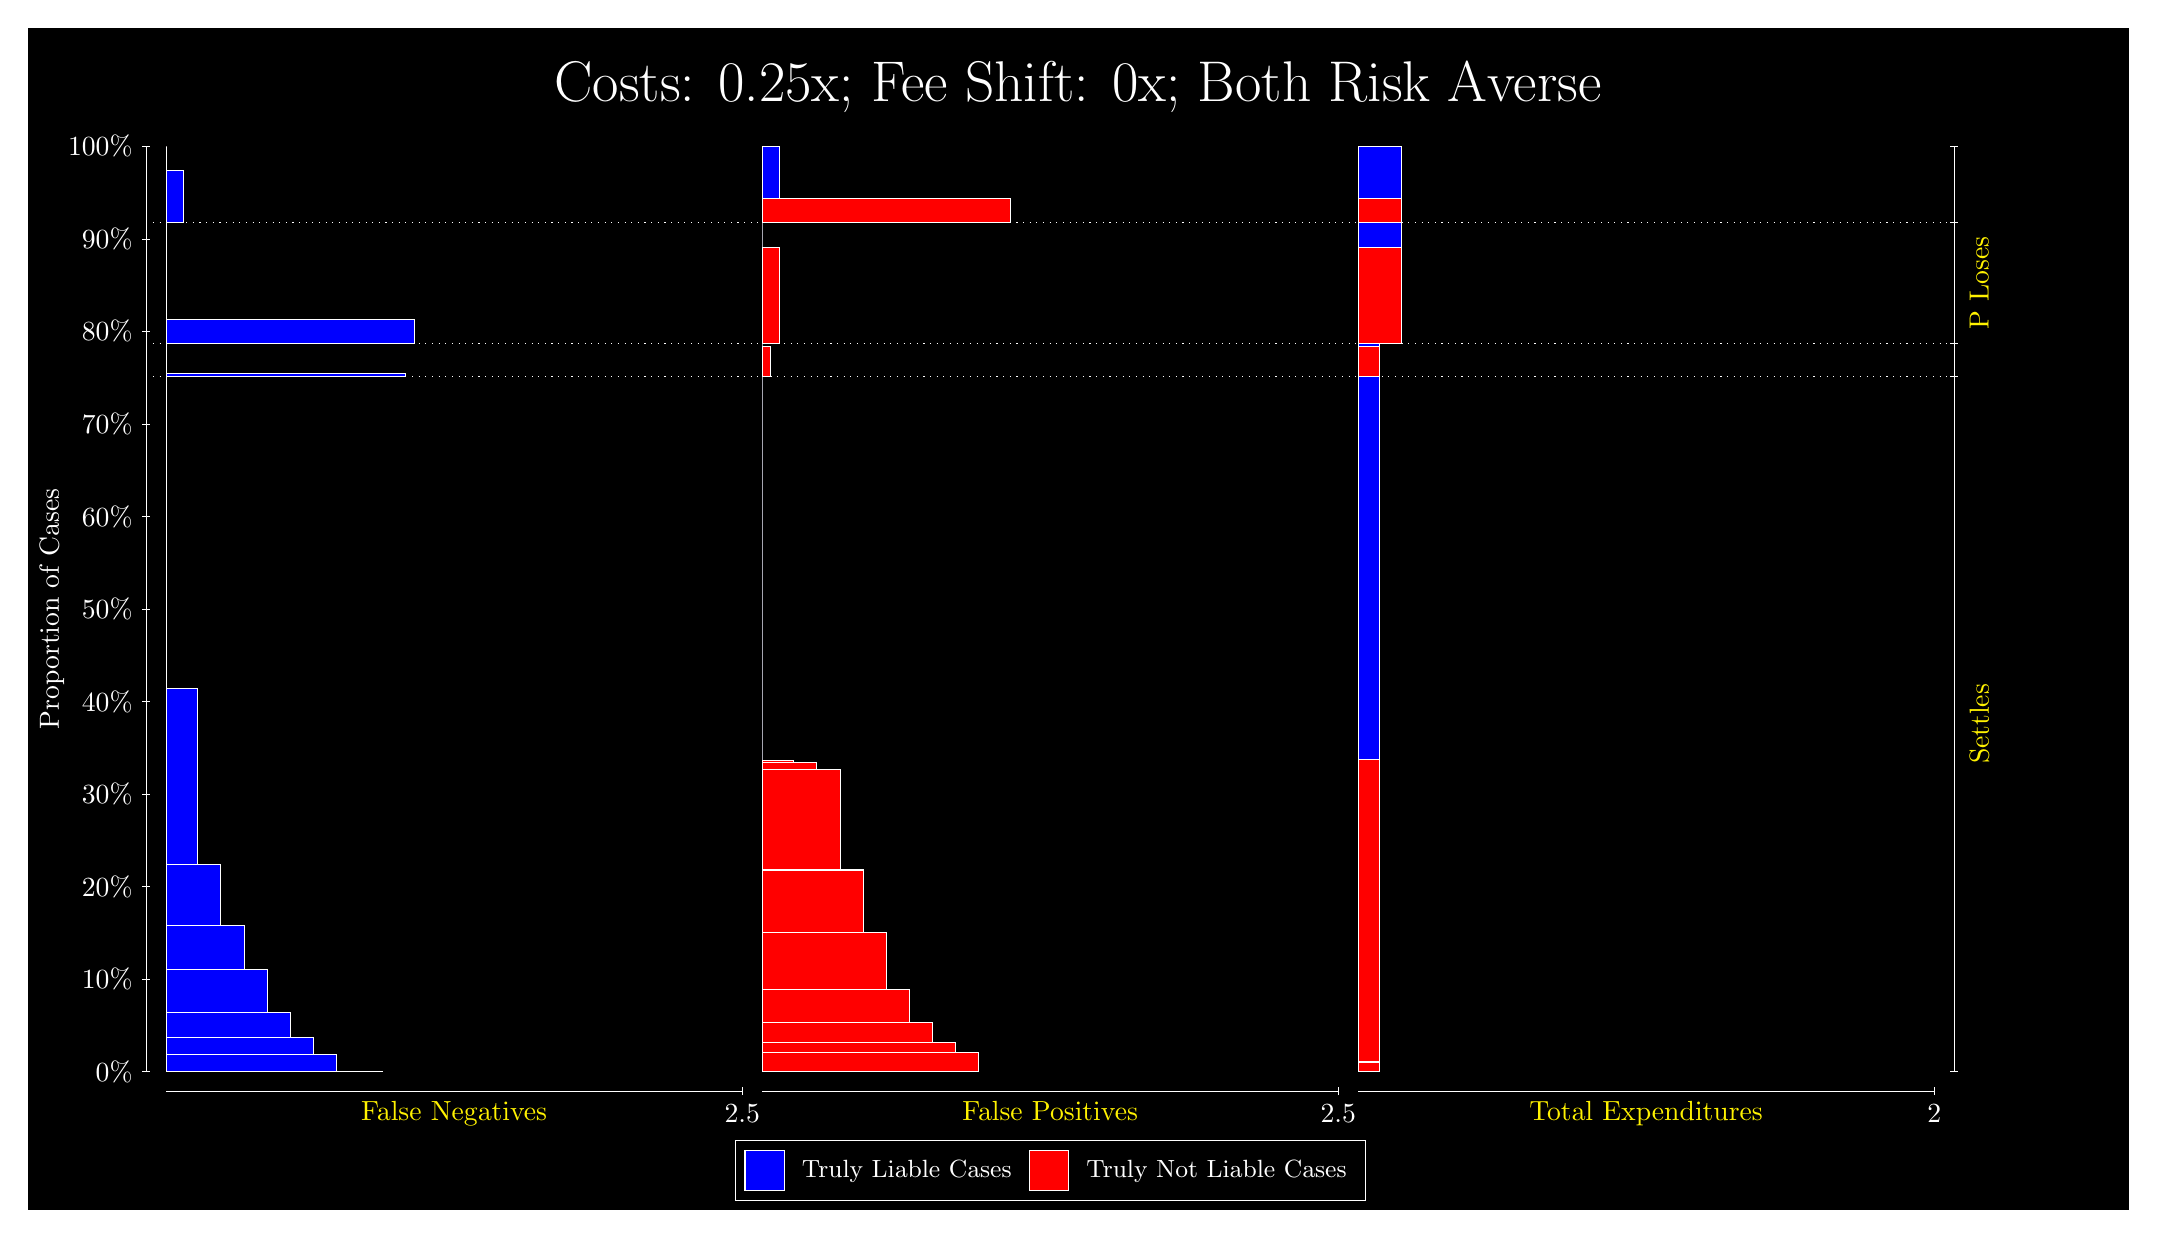
\begin{tikzpicture}
\draw[fill=black] (0,0) rectangle (26.667,15);
\draw[text=white] (0,13.5) rectangle (26.667,15) node[midway] {\huge Costs: 0.25x; Fee Shift: 0x; Both Risk Averse};
\draw[white, very thin] (1.5,1.75) -- (1.5,13.5);
\node[rotate=90, text=white, anchor=center] at (0.3, 7.625) {Proportion of Cases};
\draw[white, very thin] (1.45,1.75) -- (1.55,1.75);
\node[text=white, anchor=east] at (1.45, 1.75) {0\%};
\draw[white, very thin] (1.45,2.925) -- (1.55,2.925);
\node[text=white, anchor=east] at (1.45, 2.925) {10\%};
\draw[white, very thin] (1.45,4.1) -- (1.55,4.1);
\node[text=white, anchor=east] at (1.45, 4.1) {20\%};
\draw[white, very thin] (1.45,5.275) -- (1.55,5.275);
\node[text=white, anchor=east] at (1.45, 5.275) {30\%};
\draw[white, very thin] (1.45,6.45) -- (1.55,6.45);
\node[text=white, anchor=east] at (1.45, 6.45) {40\%};
\draw[white, very thin] (1.45,7.625) -- (1.55,7.625);
\node[text=white, anchor=east] at (1.45, 7.625) {50\%};
\draw[white, very thin] (1.45,8.8) -- (1.55,8.8);
\node[text=white, anchor=east] at (1.45, 8.8) {60\%};
\draw[white, very thin] (1.45,9.975) -- (1.55,9.975);
\node[text=white, anchor=east] at (1.45, 9.975) {70\%};
\draw[white, very thin] (1.45,11.15) -- (1.55,11.15);
\node[text=white, anchor=east] at (1.45, 11.15) {80\%};
\draw[white, very thin] (1.45,12.325) -- (1.55,12.325);
\node[text=white, anchor=east] at (1.45, 12.325) {90\%};
\draw[white, very thin] (1.45,13.5) -- (1.55,13.5);
\node[text=white, anchor=east] at (1.45, 13.5) {100\%};

\draw[white, very thin] (24.457,1.75) -- (24.457,13.5);
\draw[white, very thin] (24.407,1.75) -- (24.507,1.75);
\node[anchor=west] at (24.407, 1.75) {};
\draw[white, very thin] (24.407,10.581) -- (24.507,10.581);
\node[anchor=west] at (24.407, 10.581) {};
\draw[white, very thin] (24.407,10.993) -- (24.507,10.993);
\node[anchor=west] at (24.407, 10.993) {};
\draw[white, very thin] (24.407,12.535) -- (24.507,12.535);
\node[anchor=west] at (24.407, 12.535) {};
\draw[white, very thin] (24.407,13.5) -- (24.507,13.5);
\node[anchor=west] at (24.407, 13.5) {};

\draw[white, very thin, fill=blue] (1.75,1.75) rectangle (4.4946,1.752);
\draw[white, very thin, fill=blue] (1.75,1.752) rectangle (4.2018,1.7595);
\draw[white, very thin, fill=blue] (1.75,1.7595) rectangle (3.9091,1.9729);
\draw[white, very thin, fill=blue] (1.75,1.9729) rectangle (3.6163,2.1862);
\draw[white, very thin, fill=blue] (1.75,2.1862) rectangle (3.3236,2.5053);
\draw[white, very thin, fill=blue] (1.75,2.5053) rectangle (3.0308,3.048);
\draw[white, very thin, fill=blue] (1.75,3.048) rectangle (2.738,3.6082);
\draw[white, very thin, fill=blue] (1.75,3.6082) rectangle (2.4453,4.3817);
\draw[white, very thin, fill=blue] (1.75,4.3817) rectangle (2.1525,6.6221);
\draw[white, very thin, fill=red] (1.75,6.6221) rectangle (1.75,10.581);
\draw[white, very thin, fill=blue] (1.75,10.581) rectangle (4.7873,10.615);
\draw[white, very thin, fill=red] (1.75,10.615) rectangle (1.75,10.993);
\draw[white, very thin, fill=blue] (1.75,10.993) rectangle (4.8971,11.304);
\draw[white, very thin, fill=red] (1.75,11.304) rectangle (1.75,12.535);
\draw[white, very thin, fill=blue] (1.75,12.535) rectangle (1.9696,13.193);
\draw[white, very thin, fill=red] (1.75,13.193) rectangle (1.75,13.5);
\draw[white, very thin, fill=red] (9.3189,1.75) rectangle (12.063,1.9923);
\draw[white, very thin, fill=red] (9.3189,1.9923) rectangle (11.771,2.1201);
\draw[white, very thin, fill=red] (9.3189,2.1201) rectangle (11.478,2.3745);
\draw[white, very thin, fill=red] (9.3189,2.3745) rectangle (11.185,2.7956);
\draw[white, very thin, fill=red] (9.3189,2.7956) rectangle (10.892,3.5239);
\draw[white, very thin, fill=red] (9.3189,3.5239) rectangle (10.6,4.3005);
\draw[white, very thin, fill=red] (9.3189,4.3005) rectangle (10.6,4.3138);
\draw[white, very thin, fill=red] (9.3189,4.3138) rectangle (10.307,5.5938);
\draw[white, very thin, fill=red] (9.3189,5.5938) rectangle (10.014,5.6796);
\draw[white, very thin, fill=red] (9.3189,5.6796) rectangle (9.7214,5.7086);
\draw[white, very thin, fill=blue] (9.3189,5.7086) rectangle (9.3189,10.581);
\draw[white, very thin, fill=red] (9.3189,10.581) rectangle (9.4287,10.959);
\draw[white, very thin, fill=blue] (9.3189,10.959) rectangle (9.3189,10.993);
\draw[white, very thin, fill=red] (9.3189,10.993) rectangle (9.5384,12.224);
\draw[white, very thin, fill=blue] (9.3189,12.224) rectangle (9.3189,12.535);
\draw[white, very thin, fill=red] (9.3189,12.535) rectangle (12.466,12.842);
\draw[white, very thin, fill=blue] (9.3189,12.842) rectangle (9.5384,13.5);
\draw[white, very thin, fill=red] (16.888,1.75) rectangle (17.162,1.8648);
\draw[white, very thin, fill=blue] (16.888,1.8648) rectangle (17.162,1.8743);
\draw[white, very thin, fill=red] (16.888,1.8743) rectangle (17.162,5.7181);
\draw[white, very thin, fill=blue] (16.888,5.7181) rectangle (17.162,10.581);
\draw[white, very thin, fill=red] (16.888,10.581) rectangle (17.162,10.959);
\draw[white, very thin, fill=blue] (16.888,10.959) rectangle (17.162,10.993);
\draw[white, very thin, fill=red] (16.888,10.993) rectangle (17.437,12.224);
\draw[white, very thin, fill=blue] (16.888,12.224) rectangle (17.437,12.535);
\draw[white, very thin, fill=red] (16.888,12.535) rectangle (17.437,12.842);
\draw[white, very thin, fill=blue] (16.888,12.842) rectangle (17.437,13.5);
\draw[white, dotted] (1.5,10.581) -- (24.457,10.581);
\draw[white, dotted] (1.5,10.993) -- (24.457,10.993);
\draw[white, dotted] (1.5,12.535) -- (24.457,12.535);
\draw[white, very thin] (1.75,1.5) -- (9.0689,1.5);
\node[text=yellow, anchor=north] at (5.4094, 1.5) {False Negatives};
\draw[white, very thin] (9.0689,1.45) -- (9.0689,1.55);
\node[text=white, anchor=north] at (9.0689, 1.45) {2.5};

\draw[white, very thin] (9.3189,1.5) -- (16.638,1.5);
\node[text=yellow, anchor=north] at (12.978, 1.5) {False Positives};
\draw[white, very thin] (16.638,1.45) -- (16.638,1.55);
\node[text=white, anchor=north] at (16.638, 1.45) {2.5};

\draw[white, very thin] (16.888,1.5) -- (24.207,1.5);
\node[text=yellow, anchor=north] at (20.547, 1.5) {Total Expenditures};
\draw[white, very thin] (24.207,1.45) -- (24.207,1.55);
\node[text=white, anchor=north] at (24.207, 1.45) {2};

\node[text=yellow, centered, rotate=90] at (24.777, 6.1653) {Settles};

\node[text=yellow, centered, rotate=90] at (24.777, 11.764) {P Loses};


\draw (12.978300999999998,1.5) node[draw=none] (baseCoordinate) {};
\begin{scope}[align=center]
        \matrix[scale=0.5, draw=white, below=0.5cm of baseCoordinate, nodes={draw}, column sep=0.1cm]{
            \node[rectangle, draw, minimum width=0.5cm, minimum height=0.5cm, fill=blue] {}; &
            \node[draw=none, font=\small, text=white] (B) {Truly Liable Cases}; &
            \node[rectangle, draw, minimum width=0.5cm, minimum height=0.5cm, fill=red] {}; &
            \node[draw=none, font=\small, text=white] (B) {Truly Not Liable Cases}; \\
            };
\end{scope}

\end{tikzpicture}
\end{document}